\documentclass{article}
\usepackage{graphicx}

\title{\Large CSC 549 - Advanced Topics in Artificial Intelligence\\\large Deep Reinforcement Learning\\\normalsize Programming Assignment 3}

\author{Justin Lewis}
\begin{document}
\maketitle
\tableofcontents
\newpage
\section{Code Usage}
This is a quick description of each of the files and how to use them. 

\begin{itemize}
    \item basis.py - Useless. Meant to be a parent class
        to fourier and polynomial basis, but I didn't
        follow through very well with it. 

    \item fourier\_basis.py - Generates the coeffecient matrix and has an apply function that will apply the basis to the input. 

    \item make\_images.py - After sarsa\_lambda.py makes the numpy arrays and saves them to results, make\_images will read those in to generate the matplotlib pyplot figures for the writeup.

    \item mc.py - This is the simulation for the mountain
        car. If you run this file directly, it will render
        an animation to represent what the mountain car is
        doing. You can change between animate and animate2
        in the main function, but that's not particularly
        helpful, especially since animate2 does not have
        the offset to make the bottom of the mountain at
        the proper spot. 

    \item polynomial\_basis.py - Hypothetically correct,
        but actually using it is impractical because it
        makes the episodes very very slow. 

    \item render.py - This is a scratch file that I play around with to test things like 
        how the parameters affect the performance. Currently it's set to test a few variations
        of gamma. 

    \item numerical\_analysis.py - This is a scratch file that I play around with to test things like 
        how the parameters affect the performance. Currently it's set to test a few variations
        of gamma. 

\item sarsa\_lambda.py - \Large{This is the most interesting file!} \normalsize This one will do a bunch of runs, average them, 
    save the results to files for make\_images.py to make images for. For your sanity I recommend lowering the contants at the top of the file. 

    Parameters:
    \begin{itemize}
        \item "-\--animate" - Will run the algorithm with an animation running.
            Plays 250 frames each time (instead of stopping with the episode).
            I recommend having a run that you save the agent's weights at least
            once. Note that this only does the fourier basis with an order of
            3. 
        \item "-\--save-res" - Used to save the number of steps in an episode to files for plotting learning curves.
        \item "-\--save-w" - Used to save the average of the weights at the end of all of the runs.  
        \item "-\--load-w" - Used to load saved weights. If not found, will throw an error and exit with -1.
        % \item TODO "-\--verbose" - Does not exist, but would be nice to have verbose or maybe even verbosity levels. 
    \end{itemize}

    The ideal run cycle for your interests should be something like: 
    \begin{verbatim}
        $ python3 sarsa_lambda --save-w
           <... various output ...>
        $ python3 sarsa_lambda --load-w --animate
    \end{verbatim}
\end{itemize}

\section{Required answers}
\begin{enumerate}
    \item Learning curves, $ \epsilon = 0.03 $:

    % \begin{center}
        % 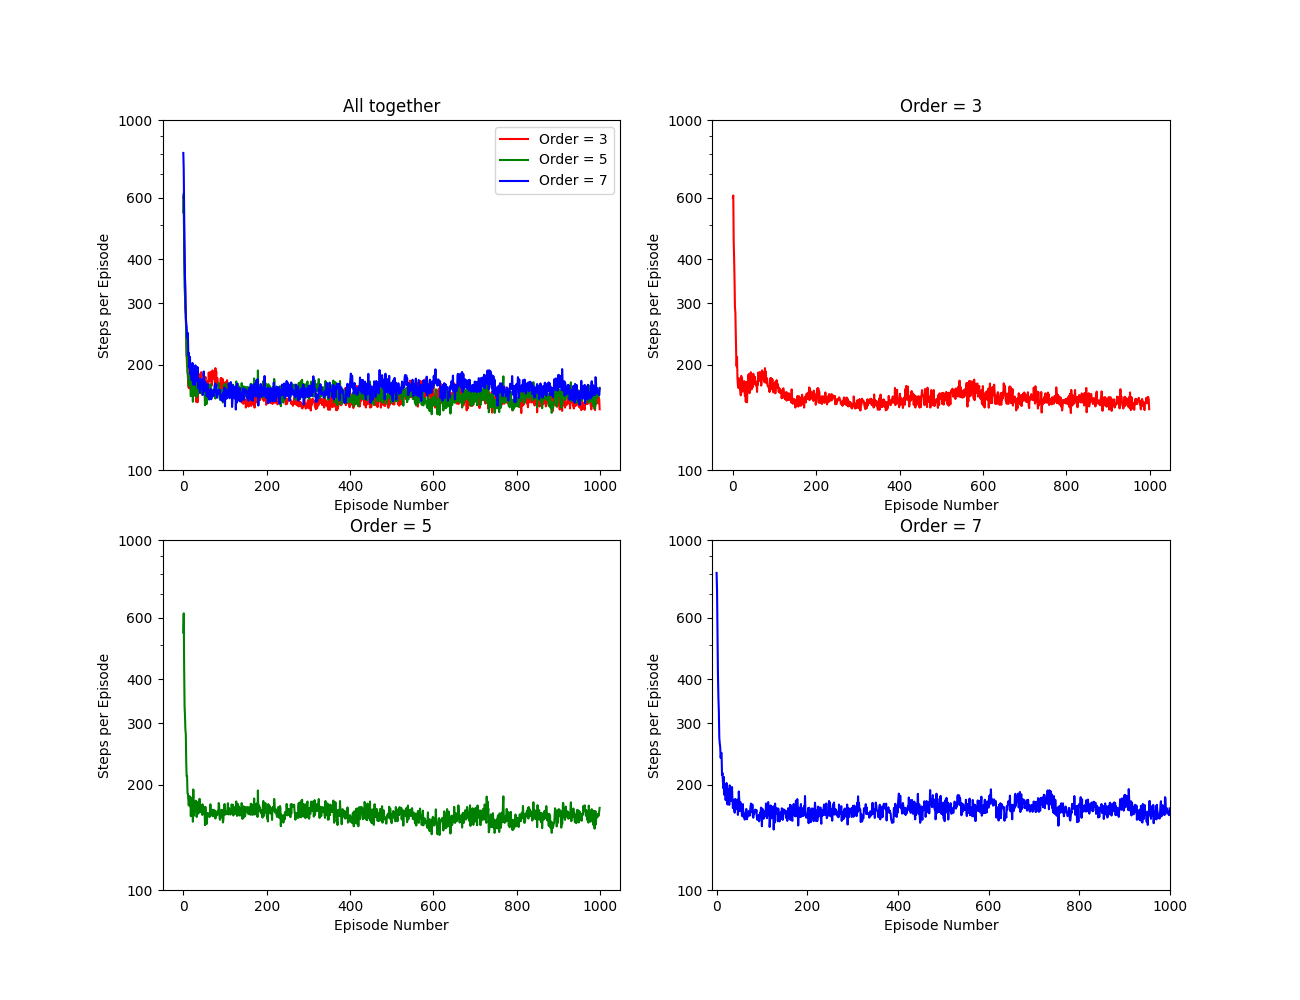
\includegraphics[width=.6\columnwidth]{images/2by2.png}
    \begin{figure}[h]
        \centerline{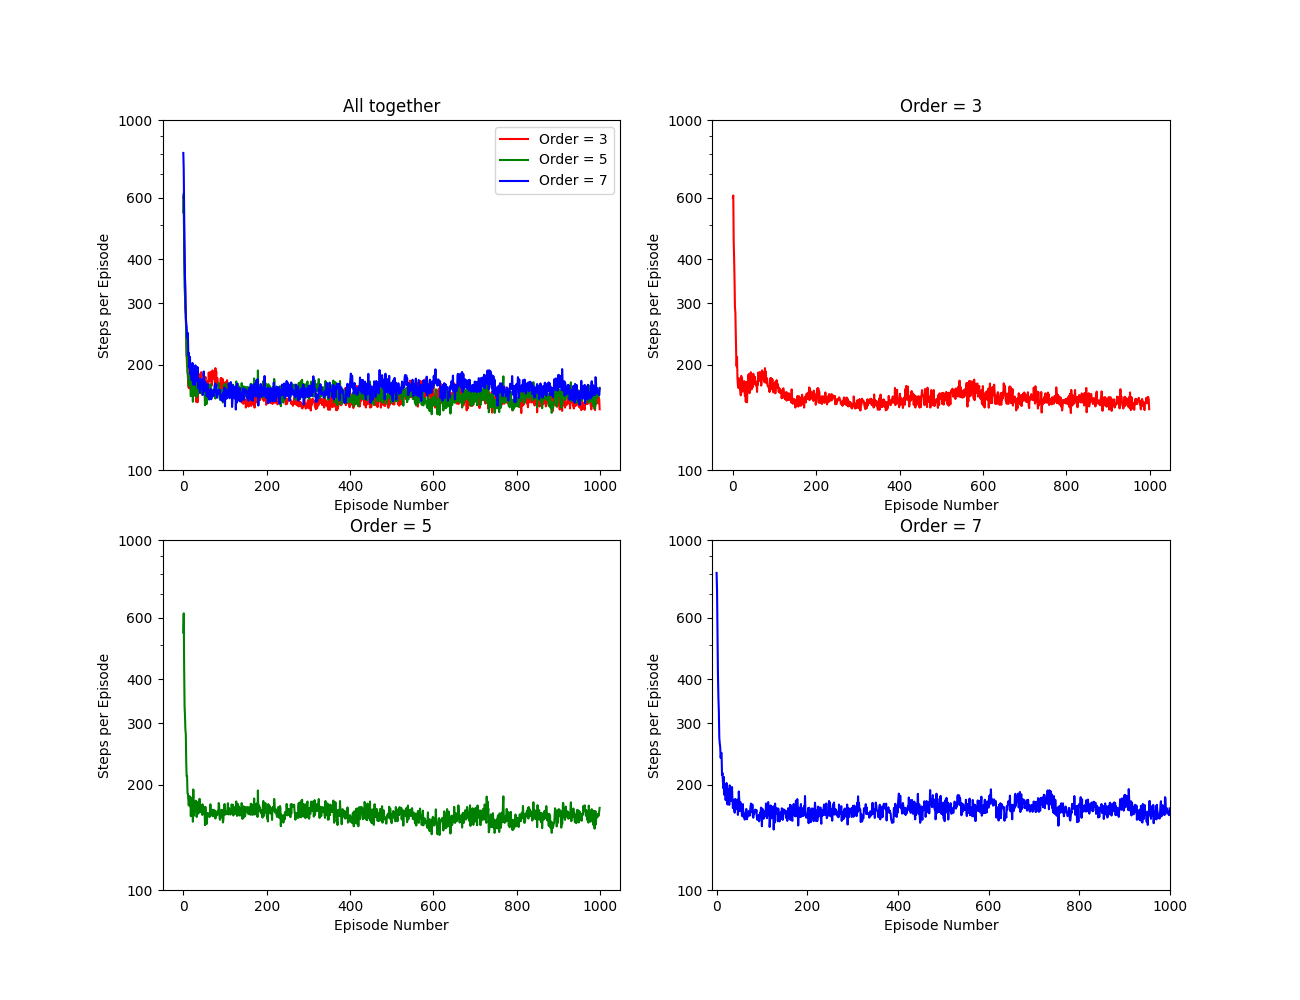
\includegraphics[width=\columnwidth]{images/2by2.png}}
    \end{figure}
    % \end{center}
    Note that while alpha is contast, it is not a scalar. 
    Alpha was set in accordance to what the research paper had their alpha, which is
    determined by the c vector of the basis:
    $$ \vec{\alpha} = \frac{0.001}{||\vec{c}||_2} $$
    This graphic shows the learning curves for orders $ 3, 5, 7 $ and $ \gamma=1, \lambda=0.9 $, 
    where $ \lambda $ is the trace decay rate and $ \gamma $ is the discount factor. 

    Based off of these graphics, it seems that the agent learns the environment ridiculously quickly. 
    I suspect that is just by nature of what a near perfect solution may be (which is to just move in the
    direction of the velocity). The agent consistently gets under 200 steps per episode after about 5 episodes, which
    I admit is rather suspeicious but I can't see anything wrong with it, I just think it's a very easy problem for the agent. 

    Anyway, to do some numerical analysis (specifically on an order of 3), it would seem the standard deviation after
    it's learned the solution is about 8 steps, with a mean of 161 steps per episode. This is very neat, and tells me that 
    a little under 70\% of the time the agent can finish the episode in $ 161 \pm 8 $ steps!

    The fastest episode (min of steps per episode) was 145 steps, and the maximum after the 25th episode was 195.45 (remember that
    this is averaged over 100 runs). 

    You can find more detailed information by looking at `numerical\_analysis.py', if you so desire. 

    In hind sight, averaging the information over 100 runs then doing this analysis somewhat ruins the point of the standard deviation\dots

\newpage

\item Surface plot of the value function. 
    I show the surface plot of all three value functions here, but they look very similar. \\
    You can look in ``make\_image.py'' for details on how these images are made.  
    \begin{figure}[h]
        \minipage{0.5\textwidth}
        \centerline{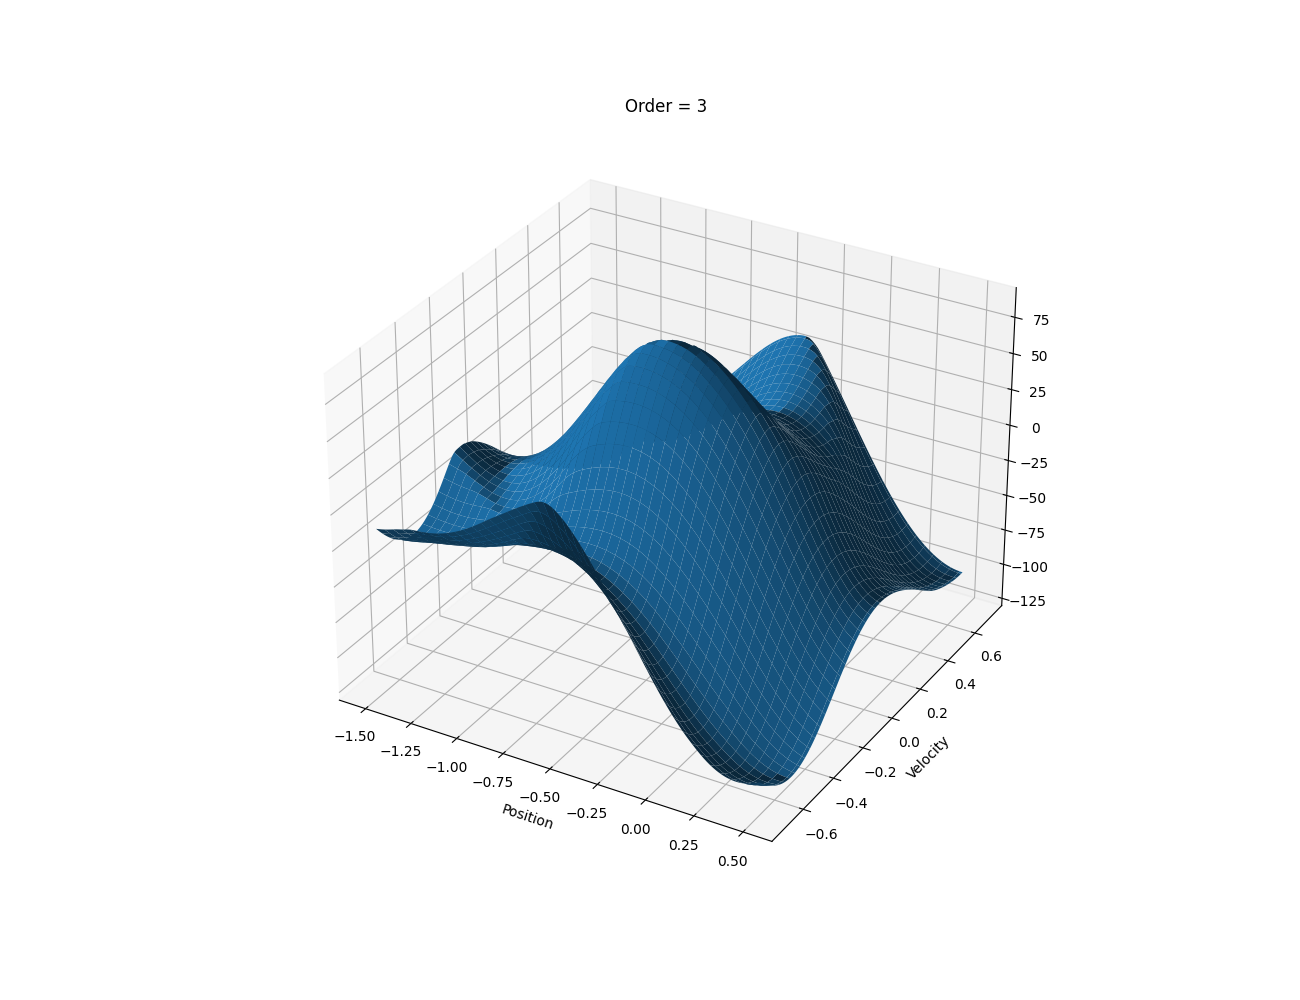
\includegraphics[width=\linewidth]{images/surfaceOrder3.png}}
            \caption{Order $ = 3 $ }
        \endminipage
        \minipage{0.5\textwidth}
        \centerline{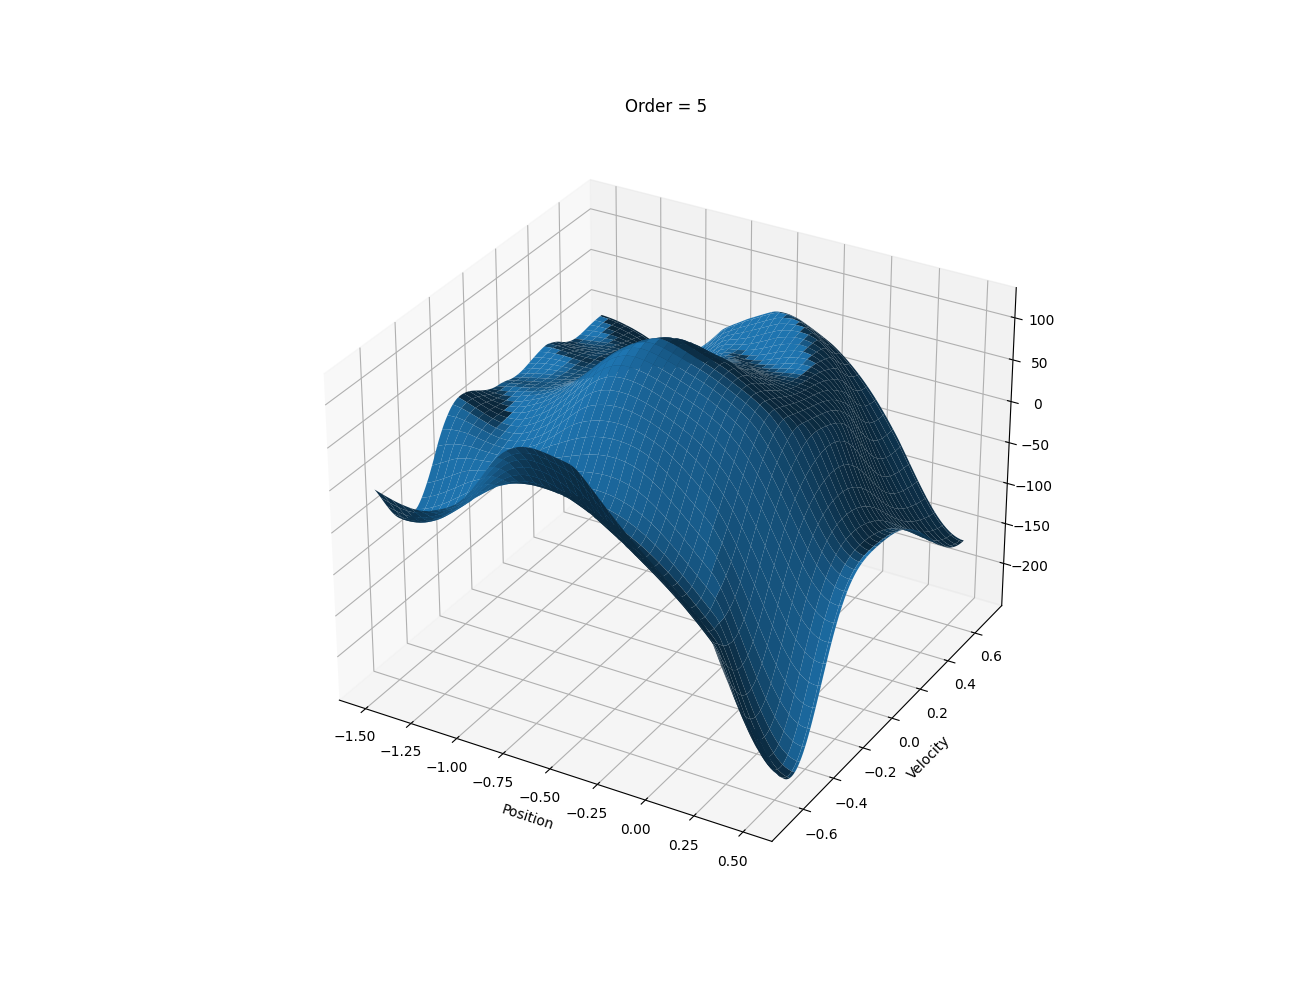
\includegraphics[width=\linewidth]{images/surfaceOrder5.png}}
            \caption{Order $ = 5 $ }
        \endminipage\hfill
    \end{figure}
    \begin{figure}[h]
        \centerline{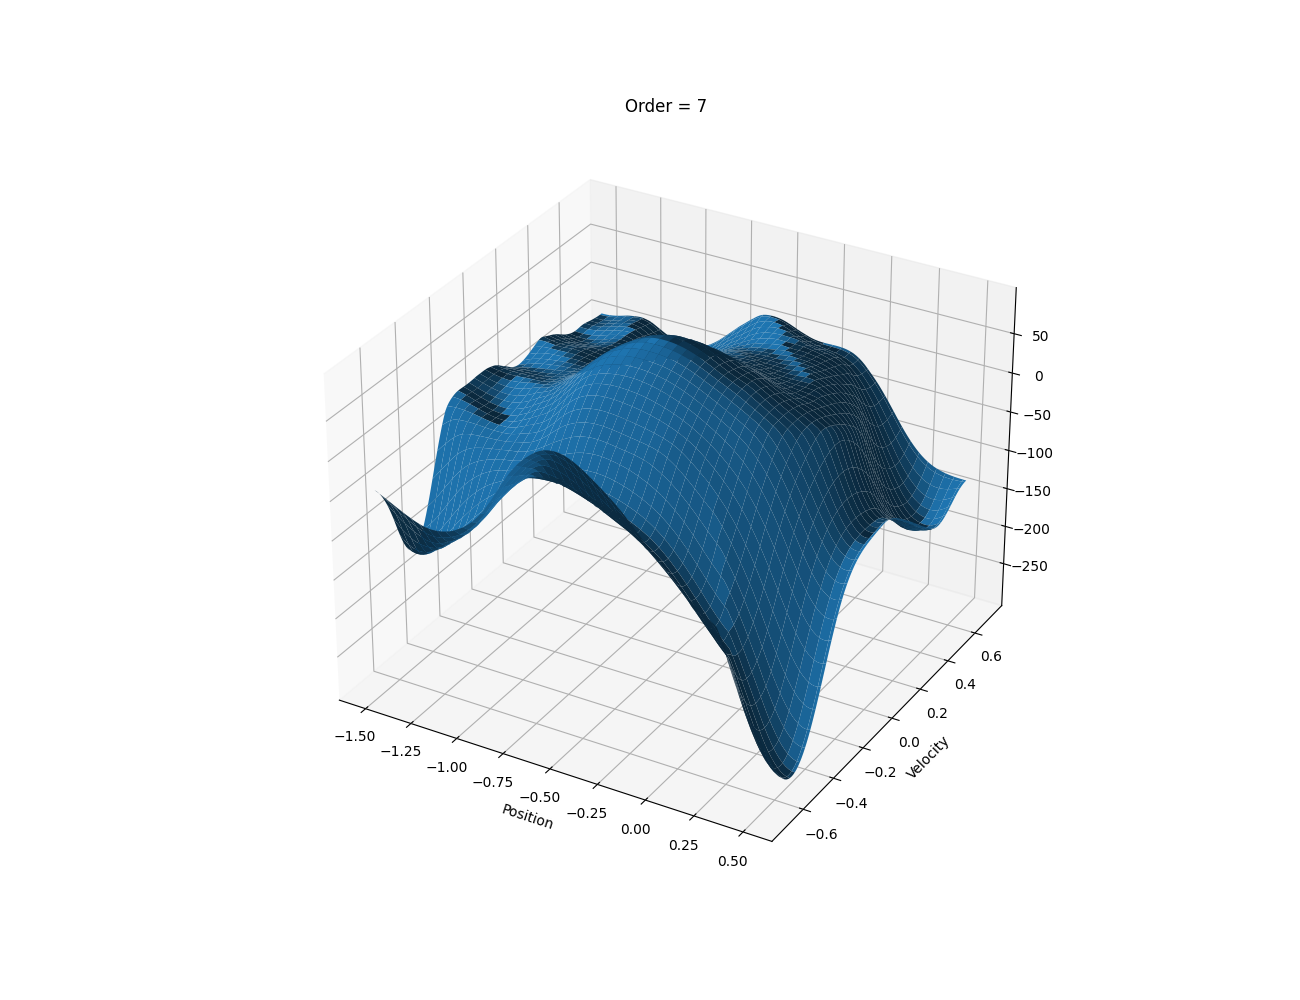
\includegraphics[width=.5\linewidth]{images/surfaceOrder7.png}}
            \caption{Order $ = 7 $ }
    \end{figure}

    I will point out that it looks different from the Sutton and Barto value function plots. 
    However, I'm confident that this is due to the face that these are rendered from an agent
    that is using a fourier basis. This can be seen in the nature of the curves, where there is a lightly visible
    periodic nature to the curves on both dimensions (which you can better see if you render it yourself and use the pyplot
    3d figure to rotate them around and see what's going on). 
    I at one point had a bug in my code where instead of calculating the value with the mesh on the proper state space, the state
    space was much too large. I didn't save any of the images, however it was very apparent the periodic nature of the bases from that. 

    Also if you just read through the paper to figure out how it works it's easy to know what's going on. The agent just learns what weights to associate
    with what cosine coefficients (not quite the right word but just the c array in fourier\_basis.py) are most relevant. Obviously by learning those the
    output is going to look similar to a cosine wave. Actually it is very similar to when you do a fourier series of a function (such as with sound processing)
    and whenever there's a proper signal at a frequency there's a spike there in the output. Very cool. 

    \newpage
\item \begin{enumerate}
    \item What would happen in $ \gamma < 1 $ and the solution was many steps long?
        When gamma is less than 1, the episodes just don't want to finish. I tested this with a gamma of .99 it finished a little slower than normal,
        but when I did 0.98 it got through very few episodes. It's also worth noting that with $ \gamma = 0.99 $, the was much more variance in the
        episode length.

        My guess at what is going on is that the gamme being lower messes with the accuracy of the Q values as well as slowing the propogation of the
        reward throught the state actions space. This seems to conflict to some degree with how the z vector is propogating the reward after getting a
        reward, but with how the gamma is applied, it seems to make sense. Running through the algorithm on a whiteboard to try to figure out what 
        is going on did not elucidate the answer to the question to me, so this is my best guess. 

        \begin{center}
    \begin{figure}[h]
        \minipage{0.5\textwidth}
        \centerline{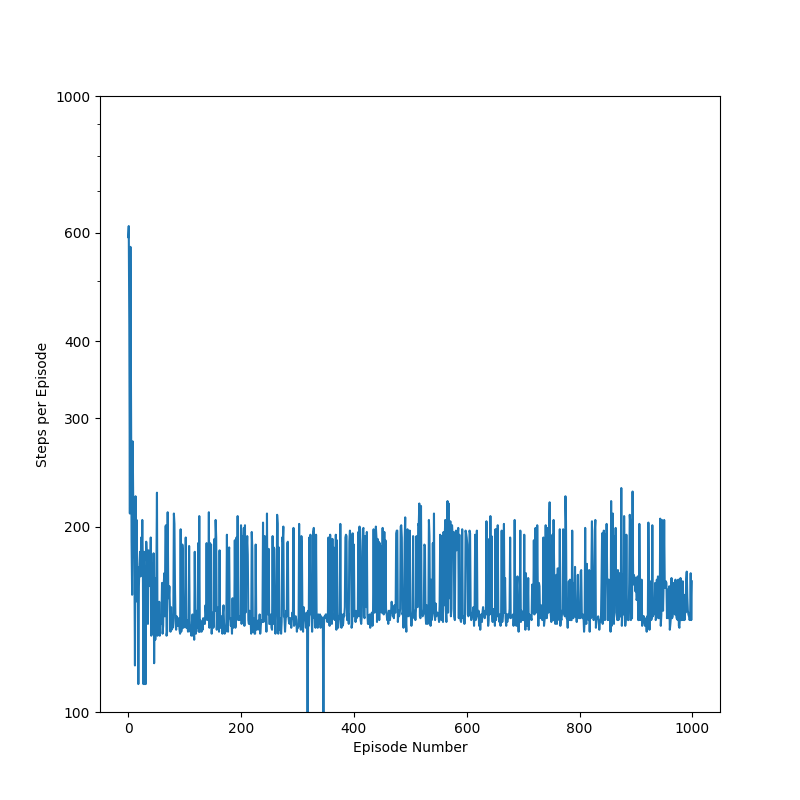
\includegraphics[width=\linewidth]{images/gamma0.png}}
            \caption{ $\gamma = 1 $ }
        \endminipage
        \minipage{0.5\textwidth}
        \centerline{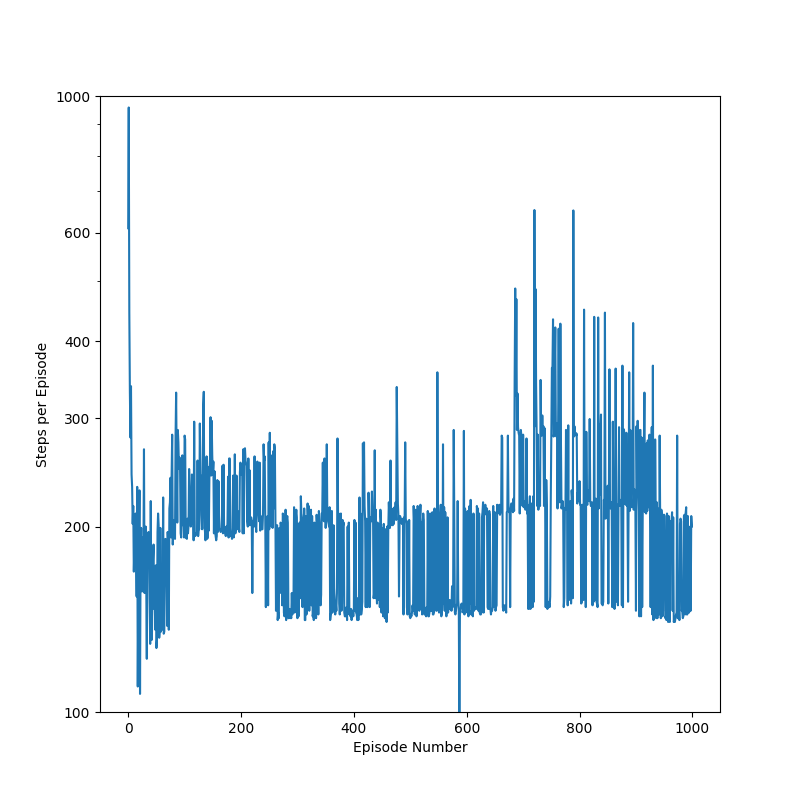
\includegraphics[width=\linewidth]{images/gamma1.png}}
            \caption{ $\gamma = .99 $ }
        \endminipage\hfill
    \end{figure}
\end{center}

    \item What would happen if we had a zero step cost and a positive goal reward, for the case
        where $ \gamma = 1 $, and the case where $ \gamma < 1 $?
        \begin{itemize}
            \item After testing this myself, for some reason after the first episode it just didn't want to finish. 
                It had gotten to nearly a million steps before I stopped it from running. 
                My guess at what is going on: 
                After the first episode (which was finished by choosing completely random actions), it only gleaned enough
                information to know that when it was on the right side of the bottom it was able to get positive reward by moving rightward. 

                This caused the agent to dislike moving left. Thus it would get as far up the hill as it could, but then once it started moving backwards it was
                essentially applying the brakes until it hit the bottom, where it would start again (since the exploration chance is too low, it never broke free
                from this). When compared against a negative reward for every action taken, even if the agent had started along the path of only trying to go right, it would have
                eventually given the state-action values enough negative values for low rightward velocities (and even negative velocities) that it realizes it needs to try going to
                the left first (which I'm fairly certain is what was always happening, even when it was initially choosing randomly, because when I made
                the change the first episode usually takes around 40000 steps. That is significantly greater than the average starting episode length of barely greater than
                1000). 

                The negative step cost apparently does wonders for teaching the agent; however I wasn't able to learn much about how gamma affects learning
                since regardless of the reward function having a gamma of less than 1 just makes the agent refuse to learn, apparently. 

            \item When $ \gamma < 1 $, the agent did nothing different. Identical results. 


        \end{itemize}
\end{enumerate}

\end{enumerate}


\section{Code base}


This section inlvolves my notes on the code involved in this assignment. 
It won't give you any value, however it will help me to gain a better
understanding of what I've done.

\subsection{Mountain Car}
I won't fully describe the code here, it is simple and you can read about the algorithm in Sutton and
Barto's Introduction to Reinforcement Learning on page 245. 

The basics is that it is meant to simulate an underpowered vehicle that needs to travel up the hill.

It simulates being underpowered by involving a $ \cos $ with the $ x $ position when you apply force to the vehice.
Underpowered is also accomplished by bounding the velocity to rather low values. 

The hill, counter-intuitively, is actually centered at roughly $ \frac{-\pi}{2}
$. To make it exactly $ - \frac{\pi}{2} $, you would need to replace the $ 3 $ in $
\cos 3 * x $ with a  $ \pi $. The reason this is counter intuitive is that it seems the cosine would
indicate where the hill is, but remember that it is actually to calculate how to manipulate the 
new velocity after applying a force. When you have the position of $ \frac{-1}{2} $, it gives the 
$ \cos{3 * x} $ a result of $ 0 $, which means it doesn't subtract anything from how the force would
affect the new velocity. You may think that it wouldn't do what you want it to
on certain positions since cosine has both negative and positive outputs, but
this actually makes it work out even better (especially with the forces
applicable including $ -1 $ and $ 1 $, which would make the signs work together
in a way that makes sense in a simulation).

\subsection{Bases}
These are wild! Basically the concept with having a fourier basis is that you're doing a kind of
fourier series on the state (where action is considered a part of the state in my implementation; an alternative
would be to have several weight vectors for each possible action, like what
Jonathan mentioned he did when I was discussing the project with him). What
this is basically doing is having the agent learn which ``harmonics'' are most
relevant to the agent to be able to figure out what it needs to do. There's a
neat trick that the paper describes where they realized they can cut the
expansion in half since the problem is ``symetric'', which I don't quite
understand but I'm guessing that it is based in the fact that the simulation
space is centered around a point (which was described in the paper) and would be just as valid to have
the goal on the left bound as the right. 

\subsection{Sarsa Lambda}
I don't have much insight to add that wasn't taught in the textbook or lectures. 

The gist if it is that the agent is learning weights for the basis function instead of the Q values for each 
state action pair, which does not scale well with continuous state (and action)
spaces. There's an eligibility trace, $ \vec{z} $, that helps the agent to more
accurately update the weights when it gets a good reward (0 in this case). 

Sadly despite my best attempts I cannot quite figure out how the linear algebra
was derived. I am unable to follow what the motivation is behind many of the calculations beyond being
able to guess at what is going on (such as $ \vec{w}^T \times \vec{x} $ would
be applying weights to the "input", to use terms I'm familiar with). 
    
\end{document}
\documentclass{article}
\usepackage{graphicx}

\title{\Large CSC 549 - Advanced Topics in Artificial Intelligence\\\large Deep Reinforcement Learning\\\normalsize Programming Assignment 3}

\author{Justin Lewis}
\begin{document}
\maketitle
